\subsection{PDFex PDF Encryption Attacks}
PDFex bezeichnet Attacken auf die PDF-Verschlüsselung mit Passwortschutz, die im Jahr 2019 entdeckt wurden. Die Forscher haben 27 PDF-Viewer auf diese Attacken getestet und alle Viewer inklusive Adobe Reader, Chrome and Firefox waren mindestens für eine Attacke anfällig. Es gibt 2 Attack-Klassifizierungen: Direct Exfiltration und \gls{cbc} malleability gadgets oder crypto gadgets genannt.
Das attacker model gestaltet sich wie folgt: 2 Personen Alice und Bob wollen ein vertrauliches PDF mit Passwortschutz austauschen. Wir nehmen an, dass ein Angreifer durch eine \gls{mitm} attack das verschlüsselte PDF unbemerkt abgreifen konnte als Alice das Dokument zu Bob geschickt hat. Daraufhin modifiziert der Angreifer das Dokument, sodass die Veränderungen unerkennbar sind für Bob, und schickt seine Version des Dokuments an Bob. Bob entsperrt das Dokument mit seinem Passwort und das entschlüsselte PDF wird automatisch zurück zum Server des Angreifers übertragen \cite{ccc-break-pdf, pdfex}.
\par

Ein verschlüsseltes PDF enthält einen Objekt-Stream als verschlüsselten ciphertext im Body und einen /Encrypt entry, der Informationen darüber enthält, wie die Daten entschlüsselt werden sollen. Der Großteil der PDF-Dateistruktur liegt unverschlüsselt vor. Ausschließlich alle Strings und Streams für Inhalte ohne die anderen Objekttypen wie Integer oder Booleans, die dokumentstrukturbeschreibend sind, werden verschlüsselt. Der Grund dafür ist, dass die PDF-Spezifikation weiterhin die random-access Optimierung im Dateiformat beibehalten möchte. Folglich ist die gesamte Dokumentenstruktur unverschlüsselt und eine ganze Reihe an wichtigen Informationen wie Anzahl und Größe der Seiten, verwendete Objekte oder Hyperlinks können vom Angreifer ausgelesen werden. \\
PDF verwendet einen speziellen Streamfilter-Typ, genannt crypt filter für die Verschlüsselung. Jeder Standard-Filter eines Streams kann vom crypt filter überschrieben werden. Ein standard identity filter wird bei besonderen Streams für z.B. Dokumentmetadaten gesetzt, damit diese in einem verschlüsselten Dokument unverschlüsselt bleiben. Diese Unterstützung von partieller Verschlüsselung kann einem Angreifer ermöglichen seinen Inhalt mit verschlüsseltem zu vermischen ohne das Passwort zu wissen. Forscher fanden 18 verschiedene Angriffsvarianten für eine ganze Reihe von PDF-Readern \cite{ccc-break-pdf}.
\par
Bei der direct exfiltration attack wird die Kryptografie nicht angerührt. Bei allen Strings im verschlüsselten PDF von Alice überschreibt der Angreifer die crypt filter mit identity filter. Jetzt kann der Angreifer bei Bedarf Strings verändern und kann weitere Objekte mit unverschlüsselten Strings hinzufügen. Außerdem kann er verschlüsselte Teile des Dokuments in Inhalte einfügen, die er kontrolliert, d.h. er kann auf verschlüsselte Streams oder Strings in seinem Inhalt referenzieren und zugreifen. Nachfolgend fügt er eine submit-form action hinzu, die Namen und Werte von AcroForms zu einer Ziel-URL überträgt. Der Text des Formularfelds wird als Stream gespeichert. Kombiniert der Angreifer eine OpenAction, die ausgeführt wird, sobald das Dokument geöffnet wird, mit einer submit-form action zu attacker.com, so kann der vertrauliche entschlüsselte Inhalt an den Angreifer zurück als POST request gesendet werden. Die OpenAction wird ausgelöst, sobald Bob sein Passwort eingegeben hat. Die direct exfiltration attack mittels submit-form action ist im PDF-Dateiformatausschnitt \ref{fig:dir-exfil} zu sehen. Statt einer sumbit-form action kann man auch einen Hyperlink oder JavaScript verwenden. Jedes Objekt kann als Hyperlink definiert werden, was einen GET request zu attacker.com triggert \cite{ccc-break-pdf, pdfex}. 
\par

\begin{figure}[!htbp]
	\centering
	\includegraphics[width=0.8\textwidth]{"images/dir\_exfilt\_forms-ccc-break-pdf.png"}
	\caption{Direct exfiltration attack mittels subit-form OpenAction \cite{ccc-break-pdf}}
	\label{fig:dir-exfil}
\end{figure}

PDF verschlüsselt durch \gls{aes}-256 mit einer Schlüssellänge von 256 Bit und operiert im \gls{cbc} mode ohne \gls{mac} Integritätsschutz. \gls{aes} gehört zu den Blockchiffren und ist ein symmetrisches Verschlüsselungsverfahren. Bei symmetrischer Verschlüsselung gibt es nur einen Schlüssel fürs Verschlüsseln und Entschlüsseln. Ein Block ist 128 Bit lang. Der subkey (Rundenschlüssel) hat immer eine Länge von 128 Bit. Die Schlüssellänge beeinflusst den key schedule, d.h. die Art und Weise wie Rundenschlüssel vom master key abgeleitet werden, sowie die Anzahl an Runden. Während der Algorithmus ausgeführt wird, wird ein 4 x 4 Array aus je 1 Byte (insgesamt 128 Bit), genannt state, in 14 Runden verschlüsselt. Im ersten einzigen Schritt, der KeyExpansion, werden die Rundenschlüssel für jede Runde plus 1 weiterer Rundenschlüssel aus dem master key berechnet. Anfangs wird der state gleichgesetzt mit dem der zu unverschlüsselten Nachricht (plaintext). Auf dem state Array wird bitweises XOR mit dem Rundenschlüssel im AddRoundKey-Schritt angewendet. Jedes Byte vom state wird dabei mit einem Byte vom Rundenschlüssel kombiniert. Die Grafik \ref{fig:aes-addk} zeigt den AddRoundKey-Schritt. Im SubBytes (substitution) Schritt wird jedes Byte des aktualisierten state Arrays mit einem Byte durch eine Substitutionstabelle (S-Box) ersetzt. Dadurch werden die Bytes im state vermischt. Eine weitere Grafik \ref{fig:aes-sub} stellt den SubBytes-Schritt dar. Danach kommt die SchiftRows-Sequenz. Die Bytes in jeder Zeile von state werden unterschiedlich nach links verschoben: Die 1. Zeile bleibt unberührt, die 2. Zeile wird um 1 verschoben, die 3. um 2 und die letzte um 3 Positionen. Die überlaufenden Zellen werden rechts an die jeweilige Zeile wieder angehängt. Im Schaubild \ref{fig:aes-shift} ist die Funktionsweise von ShiftRows gezeigt. Als Vorletztes jeder Runde außer der letzten Runde kommt MixColumns dran. Hier werden Spalten vermischt, indem jede Spalte mit einer konstanten Matrix zu einer neuen Spalte multipliziert wird. Anschaulich wird MixColumns im Schaubild \ref{fig:aes-mix} graphisch umgesetzt. Abschließend zu jeder Runde wird nochmals AddRoundKey mit dem aktuellen Rundenschlüssel ausgeführt, also state bitweise XOR verknüpft mit dem Rundenschlüssel. Im letzten Schritt produziert AddRoundKey den ciphertext. Die invertierte Operation des Algorithmus wird beim entschlüsseln angewendet und alle Funktionen werden umgekehrt aufgerufen \cite{intro-crypto, studyflix-aes, simply-aes}. \\

\begin{figure}[!htbp]
	\centering
	\includegraphics[width=0.7\textwidth]{"images/aes\_addroundkey.png"}
	\caption{AddRoundKey-Schritt im \gls{aes}-Algorithmus \cite{wiki-aes}}
	\label{fig:aes-addk}
\end{figure}

\begin{figure}[!htbp]
	\centering
	\includegraphics[width=0.7\textwidth]{"images/aes\_subbytes.png"}
	\caption{SubBytes-Schritt im \gls{aes}-Algorithmus \cite{wiki-aes}}
	\label{fig:aes-sub}
\end{figure}

\begin{figure}[!htbp]
	\centering
	\includegraphics[width=0.7\textwidth]{"images/aes\_shiftrows.png"}
	\caption{ShiftRows-Schritt im \gls{aes}-Algorithmus \cite{wiki-aes}}
	\label{fig:aes-shift}
\end{figure}

\begin{figure}[!htbp]
	\centering
	\includegraphics[width=0.7\textwidth]{"images/aes\_mixcolumns.png"}
	\caption{MixColumns-Schritt im \gls{aes}-Algorithmus \cite{wiki-aes}}
	\label{fig:aes-mix}
\end{figure}

Während des \gls{cbc} mode wird ein vorheriger ciphertext block mit dem nächsten plaintext block durch XOR verknüpft. Das Ergebnis und der Schlüssel dienen als Input für den \gls{aes}-Algorithmus und produzieren den verschlüsselten Output als ciphertext block. Außerdem wird der Output des vorherigen Blocks (ciphertext) als Input für die XOR-Verknüpfung des nächsten Blocks (plaintext) wiederverwendet. Im ersten Schritt wird der erste plaintext block mit einem Initialisierungsvektor IV (nonce) als Zufallszahl oder Zeitstempel mit XOR verknüpft. IV sollte nur einmal verwendet werden und wird dem Empfänger vom Sender mit dem ciphertext übertragen, jedoch muss IV nicht geheim bleiben. Bei mindestens einer Bitmanipulation oder einem einzigen Bitfehler im ciphertext block werden die Entschlüsselung diese Blocks und alle nachfolgenden Blöcke beeinflusst. Grafik \ref{fig:cbc} zeigt das Prinzip von Verschlüsselung und Entschlüsselung im \gls{cbc} mode. \\

\begin{figure}[!htbp]
	\centering
	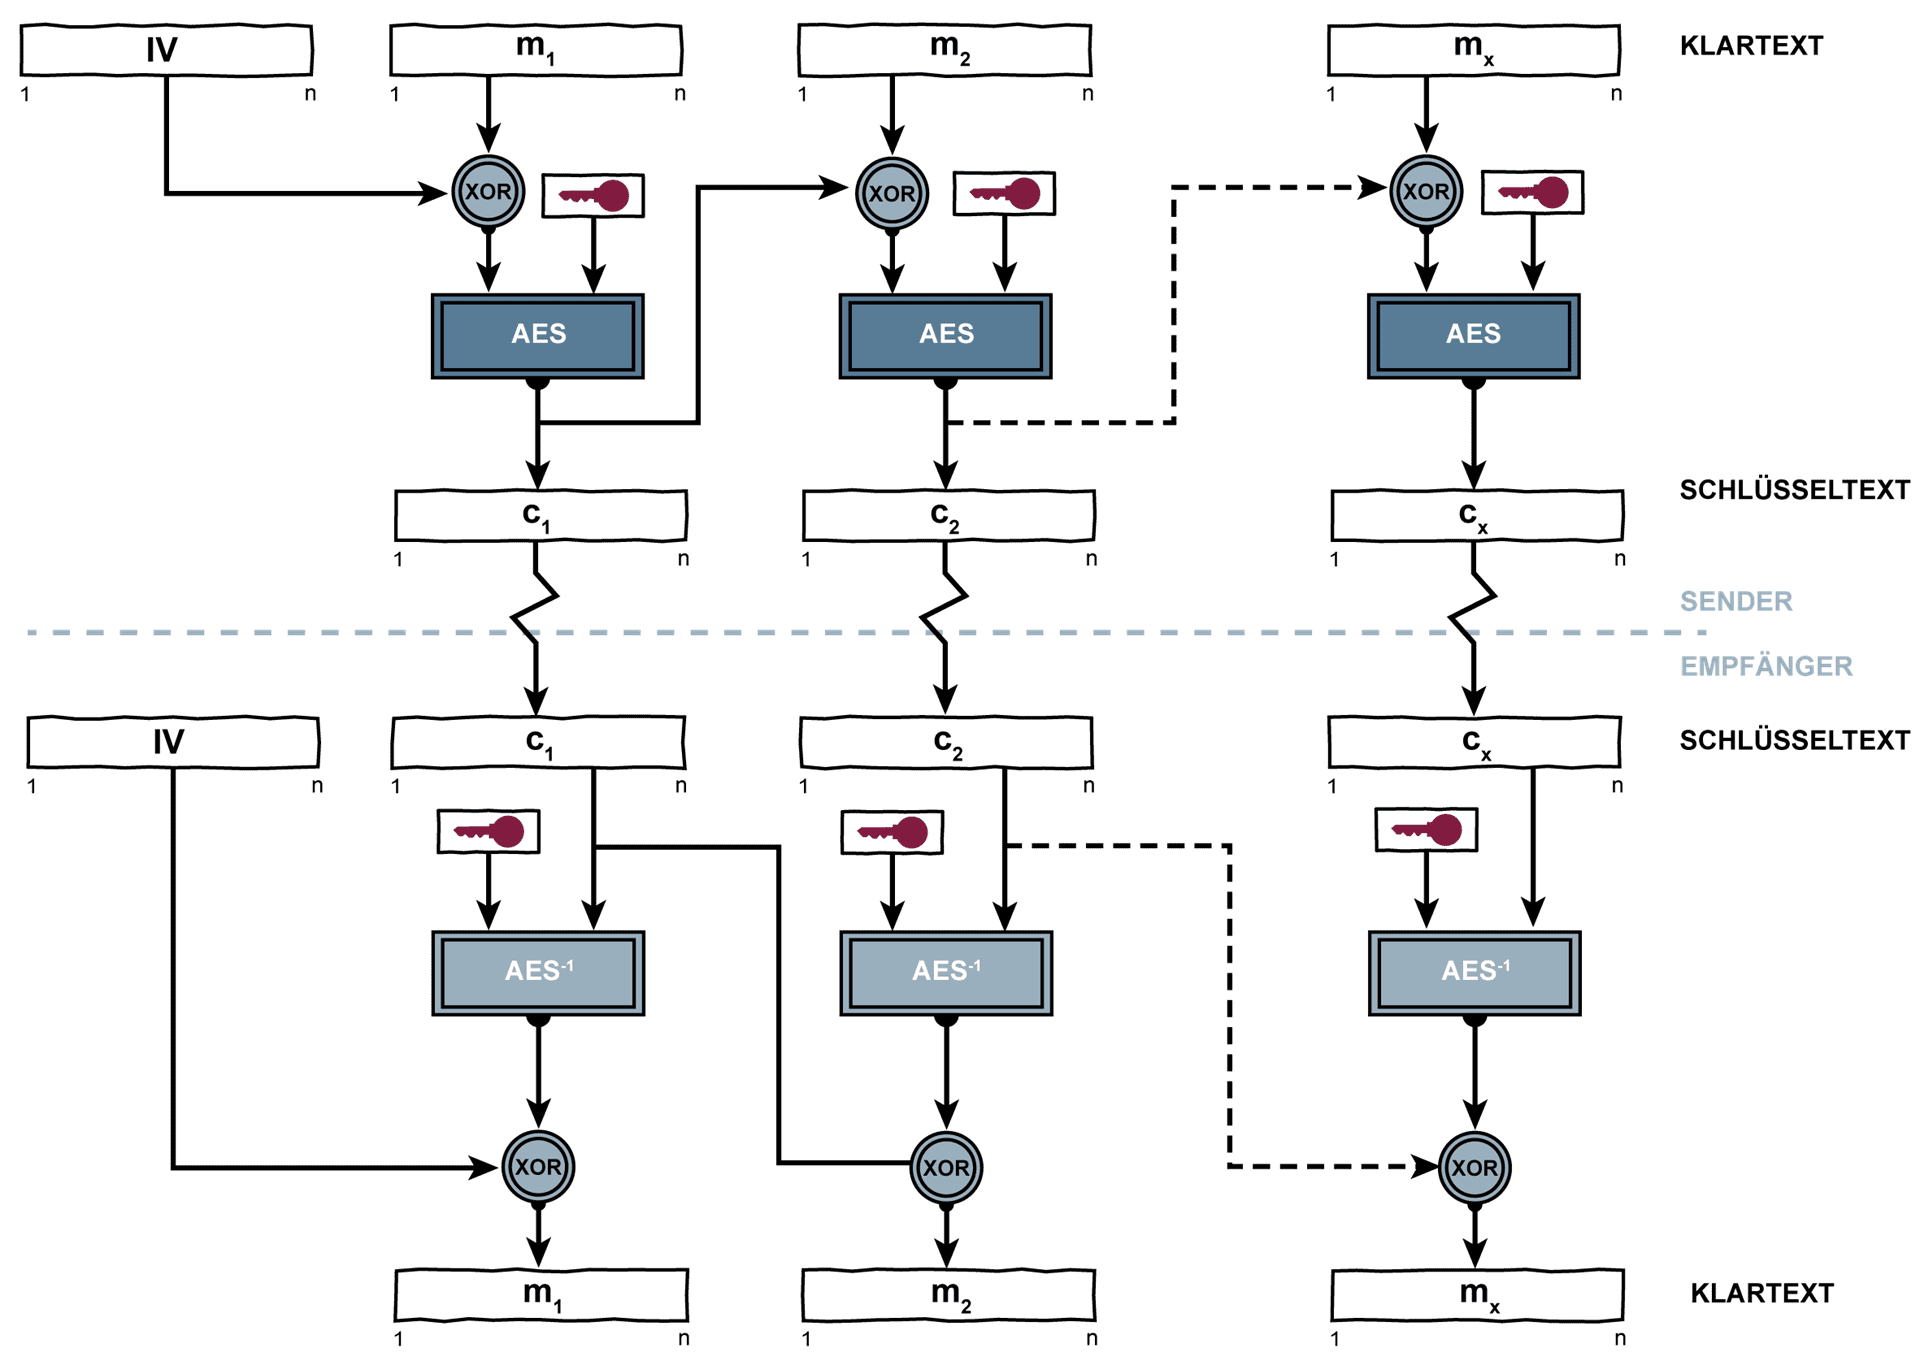
\includegraphics[width=0.8\textwidth]{"images/cbc.png"}
	\caption{\gls{cbc} mode Verschlüsselung und Entschlüsselung \cite{cbc}}
	\label{fig:cbc}
\end{figure}

Ein \gls{mac} ist eine kryptographische Prüfsumme, die aus dem Datensatz und dem symmetrischen Schlüssel von Sender und Empfänger gebildet wird. Im Gegensatz zu einem Hash kann der \gls{mac} nur von Sender und Empfänger berechnet und ebenfalls von beiden verifiziert werden \cite{crypto-web}.
\par
Nicht alle PDF-Viewer unterstützen teilweise verschlüsselte Dokumente. Solche Viewer sind immun gegen direct exfiltration attacks. Trotzdem können Angreifer \gls{cbc} malleability gadgets verwenden, um die Exfiltration des Texts zu erhalten, da keine \gls{mac} für den ciphertext beim PDF-Standard verwendet wird. Für die Ausführung der Attacke müssen 2 Vorbedingungen erfüllt sein: Zum einen muss ein plaintext-Segment dem Angreifer vorliegen. Beim aktuellsten \gls{aes}V3-Algorithmus kann der plaintext als 16 Bytes aus dem verschlüsselten /Perms entry (extended permissions) einer PDF-Datei abgeleitet werden. Die zweiten 4 Bytes sind die permissions /P, die unverschlüsselt im PDF-Dokument herausgelesen werden können. Das Byte aus T oder F wird entsprechend des EncryptMetadate Booleans gesetzt. Abschließend kommen 3 Konstante characters "adb" und 4 random Bytes. Die Tabelle \ref{table:perms} bietet eine Übersicht des /Perms entries. Der /Perms entry wird mit dem gleichen Schlüssel für Streams und Strings verschlüsselt, daher kann man ihn verwendet um \gls{cbc} gadgets zu konstruieren. Obwohl der /Perms-Wert mit \gls{ecb} mode verschlüsselt wird, ist der output ciphertext gleich seinem plaintext, wenn man ihn mit \gls{cbc} verschlüsselt und dabei einen initialization vector von 0 verwendet würde. Bei älteren Versionen des \gls{aes}-Algorithmus in PDF muss der bekannte plaintext aus dem Objekt, auf das die Exfiltration angewendet werden soll, extrahiert werden \cite{ccc-break-pdf, pdfex}.

\begin{table}[!htbp]
	\centering
	\begin{tabular}{|p{2cm}|p{2cm}|p{2cm}|p{2cm}|p{2cm}|}
	\hline
	\textbf{1...1}	& \textbf{PValue} 	& \textbf{"'T"'/"'F"'} 	& \textbf{"'adb"'} 	& \textbf{random} 	\\ 
	\hline
	4 byte 			& 4 byte 			& 1 byte  			& 3 byte 			& 4 byte 			\\ 
	\hline
	\end{tabular}
	\caption{Bytebelegung beim /Perms (extended persmissions) entry in einer verschlüsselten PDF-Datei \cite{ccc-break-pdf}}
	\label{table:perms}
\end{table}

Alice verschlüsselt eine Nachricht aus 2 Blöcken p0 und p1 zum initialization vector IV, c0 und c1 und Bob kann diese Nachricht wieder zu p0 und p1 entschlüsseln. \gls{cbc} gadgets kann man konstruieren mit einem bekannten plaintext (known plaintext) von 16 Bytes p0 und kann dadurch vom Angreifer ausgewählte plaintext blocks (chosen plaintext) g0 und g1 in eine entschlüsselte plaintext message einfügen. Beispielsweise könnte g1 die URL vom Angreifer enthalten, sodass er sich die entschlüsselte Nachricht p1 von Bob zu seinem Server schicken lassen kann. Der Angreifer erhält die verschlüsselte Nachricht aus IV, c0 und c1 von Alice durch eine \gls{mitm} attack und konstruiert 2 neue initialization vectors x0 und x1. Nimmt man IV XOR p0 erhält man ausschließlich Nullen. X0 als vom Angreifer erstellter IV wird durch IV XOR p0 XOR g0 und x1 als zweiter vom Angreifer erstellter IV wird durch IV XOR p0 XOR g1 gebildet. Eine neue verschlüsselte Nachricht wird durch die Konkatenation von x0, c0, x1, c0 und c1 gebildet. Der ursprüngliche c0 Block wird 2 Mal verwendet. X0 und x1 sind die neuen IV und x1 ist lediglich an dieser Stelle zwischen c0 in der Verkettung, um sie beizubehalten. X1 wird zu unkontrollierbaren Bytes ohne Sinn entschlüsselt. C1 ist der ciphertext block von Alice, der die Zieldaten, enthält. Bei der Entschlüsselung erhält Bob den chosen plaintext block g0, die unkontrollierten Bytes, den zweiten chosen plaintext block g1 und die entschlüsselten Zieldaten von Alice p1. Abbild \ref{fig:gadget} zeigt das Wirkungsprinzip von \gls{cbc} gadgets. Als Exfiltration Channel kommen AcroForms oder Hyperlinks in Frage, um die entschlüsselte Nachricht von Bob zurück an den Angreifer zu schicken \cite{gadget, ccc-break-pdf, crypto-web}.
\par

\begin{figure}[!htbp]
	\centering
	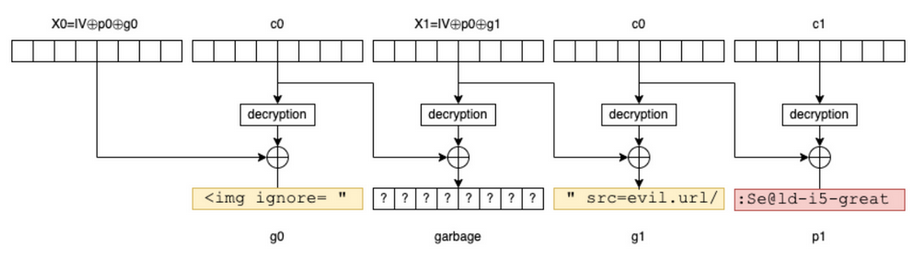
\includegraphics[width=1\textwidth]{"images/gadget2-gadget.png"}
	\caption{\gls{cbc} malleability gadget mit konstruierten initialization vectors x0 und x1, um chosen plaintext einzuschleusen \cite{gadget}}
	\label{fig:gadget}
\end{figure}

Hauptursache des Problems ist, dass viele Datenformate eine Teilverschlüsselung erlauben, z.B. \gls{xml}, S/\gls{mime} und PDF, was dem Angreifer ermöglicht eigene Inhalte einzuschleusen und exfiltration channels bilden zu können. Des Weiteren enthält \gls{aes}-\gls{cbc} keinen Integritätsschutz wie einen \gls{mac}, sogar nicht in PDF 2.0. Diese Sicherheitslücken sollten ohne Rückwärtskompatibilität in zukünftigen PDF-Spezifikationen entfernt werden \cite{pdfex}.
